% !TEX program = xelatex
\documentclass[12pt, a4paper]{article}
\usepackage[utf8]{inputenc}

\usepackage{fontspec}
\setmainfont[Ligatures=TeX]{Linux Libertine O}

\usepackage[hidelinks, colorlinks = true, linkcolor = black, urlcolor = blue]{hyperref}
\usepackage{indentfirst}
\usepackage{graphicx}
\graphicspath{{opamp/}}
\usepackage[left=1cm,right=1cm,top=2cm,bottom=2cm]{geometry}
\usepackage{lipsum}
\usepackage{caption}
\usepackage{subcaption}
\usepackage{dirtytalk}
\usepackage{amsmath}
\usepackage[framed,numbered,autolinebreaks,useliterate]{mcode}


\title{\textbf{Ηλεκτρονική 3} \\ \textbf{Αναφορά Εργαστηρίου}}
\author{Θεόδωρος Κατζάλης \\ ΑΕΜ:9282 \\ katzalis@auth.gr}
\date{15 Ιανουαρίου 2021}


\begin{document}

\maketitle
\sloppy
\tableofcontents
\pagebreak

\section{Άσκηση 1}

Η άσκηση 1 αναφέρεται στην δημιουργία τάσης τριγωνικής κυματομορφής μέσω της σύνθεσης δύο επιμέρους κυκλωμάτων. Έχουμε δύο τελεστικούς ενισχυτές όπου ο ένας λειτουργεί ως πολυδονητής (συνδεσμολογία συγκριτή) και ο δεύτερος ως ολοκληρωτής. Η αντίσταση  R2 είναι αντίσταση προστασίας για τις zener, ο ρόλος των οποίων είναι να κρατάνε σε σταθερή τιμή την τάση V2. Η τιμή της V2 χωρίς τις zener δεν θα παρέμενε σταθερή σε περίπτωση που αλλάζε η τροφοδοσία του ενισχυτή. Αυτή η αλλαγή θα επηρέαζε την τάση και τον χρόνο φόρτισης του πυκνωτή το οποίο θα επηρεάζε και αυτό με την σειρά του την κλίση της κυματομορφής που θα παίρναμε στην έξοδο.



\begin{figure}[h!]
	\centering
	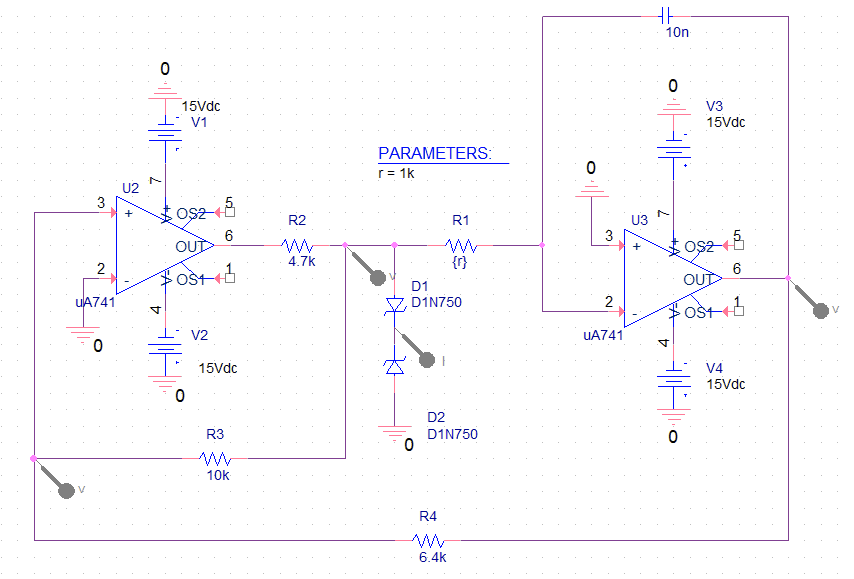
\includegraphics[width = \textwidth, height = .35\textheight, keepaspectratio]{lab/assets/exe1circuit.png}
	\caption{Κύκλωμα γεννήτριας τριγωνικών κυματομορφών}
\end{figure}


\subsection{Ερώτημα 4}

\begin{figure}[h!]
    \centering
	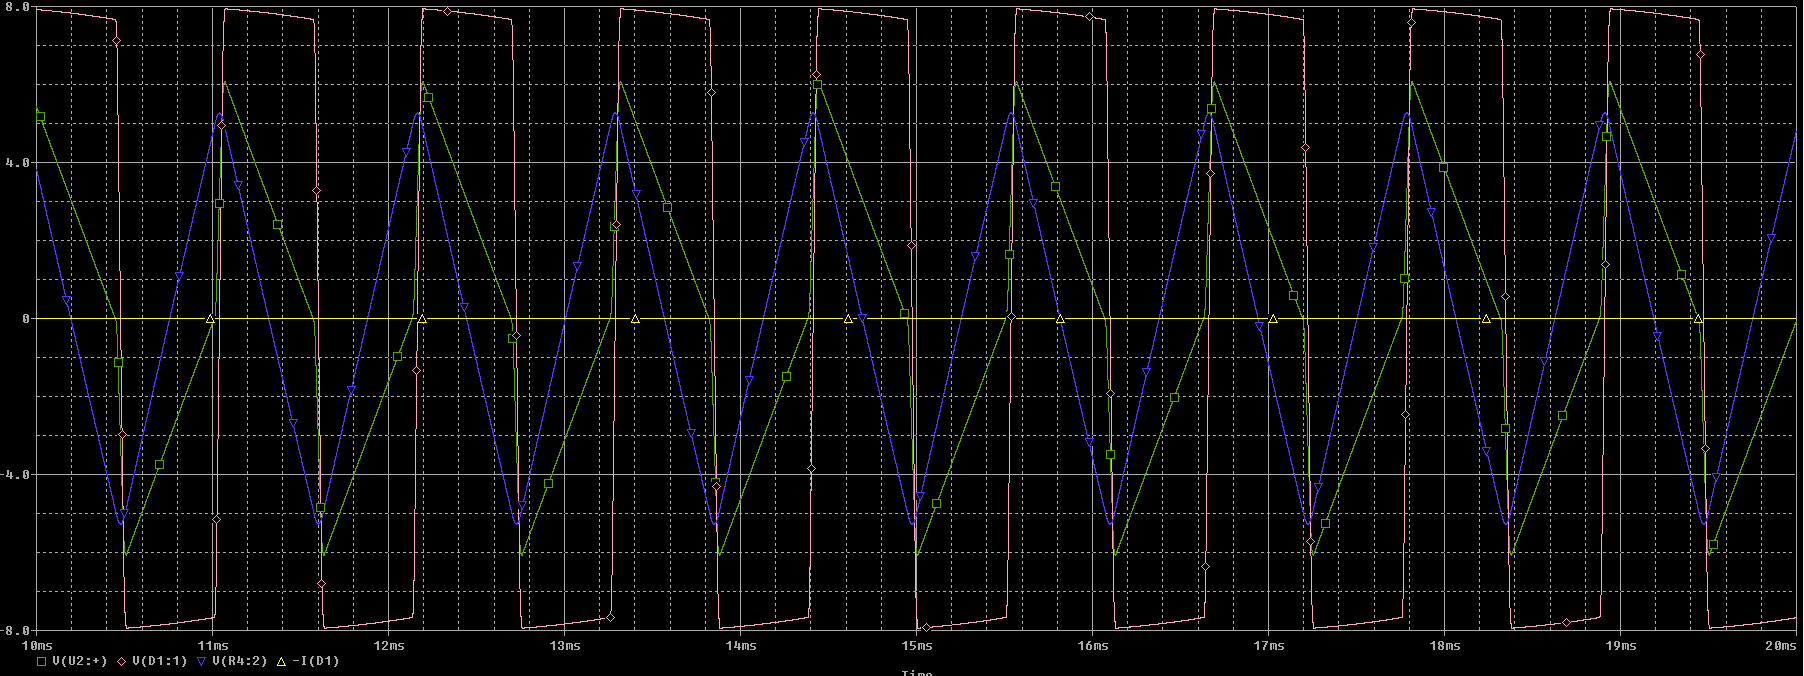
\includegraphics[width = \textwidth, height = .25\textheight, keepaspectratio]{lab/assets/gentri1.png}
    \caption{R2 = 4.7k}
\end{figure}

Παρατηρούμε ότι η V1 είναι το αλγεβρικό άθροισμα των Vout και V2 και ότι η V2 δεν είναι ένας καθαρός τετραγωνικός παλμός, υπάρχει μια μικρή κλίση.

%Το ρεύμα της zener: $Ι_z = 87.84 pA$


\subsection{Ερώτημα 5}

Πραγματοποιούμε παραμετρική ανάλυση για 1k έως 101k με step 20k για την αντίσταση R και βλέπουμε την $V_{out}$ και την $V_2$ προκειμένου να βρούμε την μέγιστη συχνότητα λειτουργίας, δηλαδή πότε ο τετραγωνικός παλμός αρχίζει πλέον και παραμορφώνει ή για ποιά τιμή οι κορυφές της τριγωνικής κυματομορφής αρχίζουν και καμπυλώνουν. Επειδή δεν είναι πολύ σαφές πότε αλλοιώνεται το "γόνατο" του τετραγωνικού παλμού θα εστιάσουμε την προσοχή μας στις κορυφές των τριγώνων. Με βάση τα παρακάτω γραφήματα μπορούμε να ισχυριστούμε ότι για 61k αρχίζει η αλλοίωση τους. Οπότε για αυτήν την τιμή της αντίστασης βλέπουμε τον τριγωνικό παλμό και έχουμε $f_{max} = 1/T_{max} = 1/1.7ms \approx 600H$.


\begin{figure}[h!]
    \centering
    \centering
	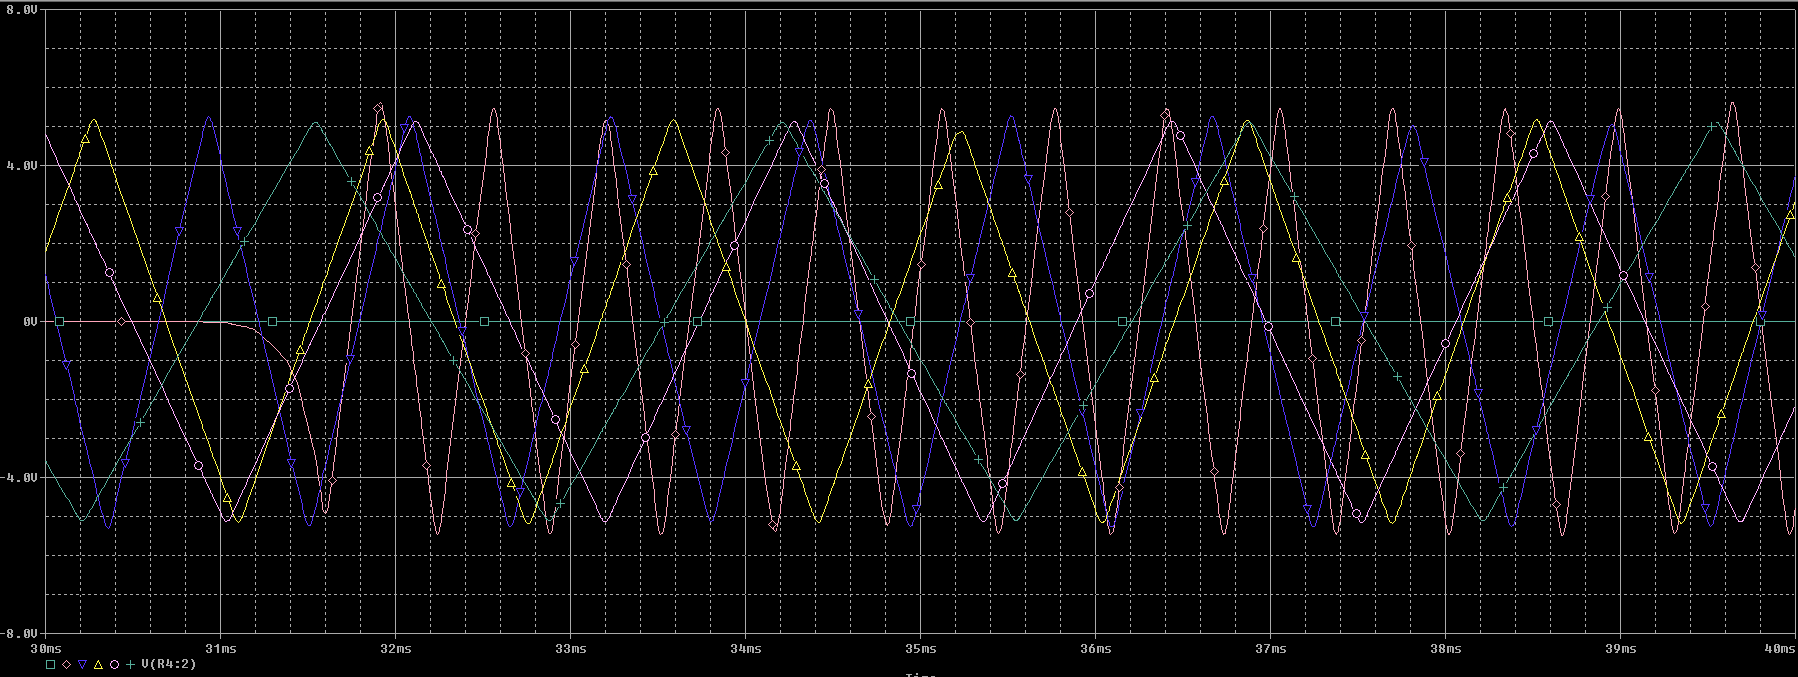
\includegraphics[width = \textwidth, height = .25\textheight, keepaspectratio]{lab/assets/gentri3.png}
    \caption{R2 = 4.7k}
\end{figure}


\begin{figure}[h!]
    \centering
	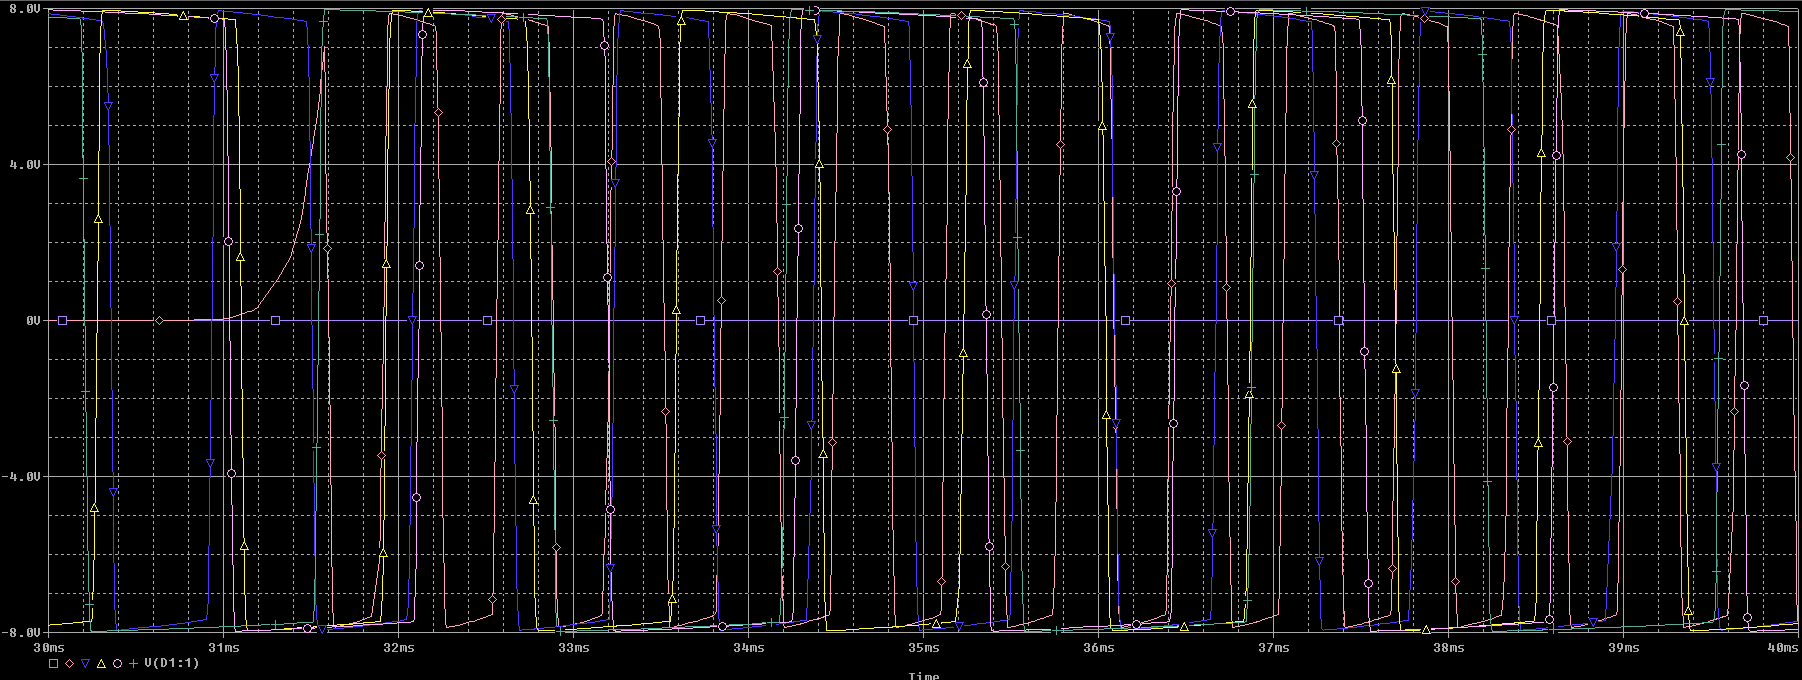
\includegraphics[width = \textwidth, height = .25\textheight, keepaspectratio]{lab/assets/gentri4.png}
    \caption{R2 = 4.7k}
\end{figure}

\pagebreak

\subsection{Ερώτημα 6}

Πραγματοποιούμε τις ίδιες παραμετρικές αναλύσεις του ερωτήματος 5 για την τιμή R2 = 1k και έχουμε τα εξής γραφήματα:


\begin{figure}[h!]
    \centering
	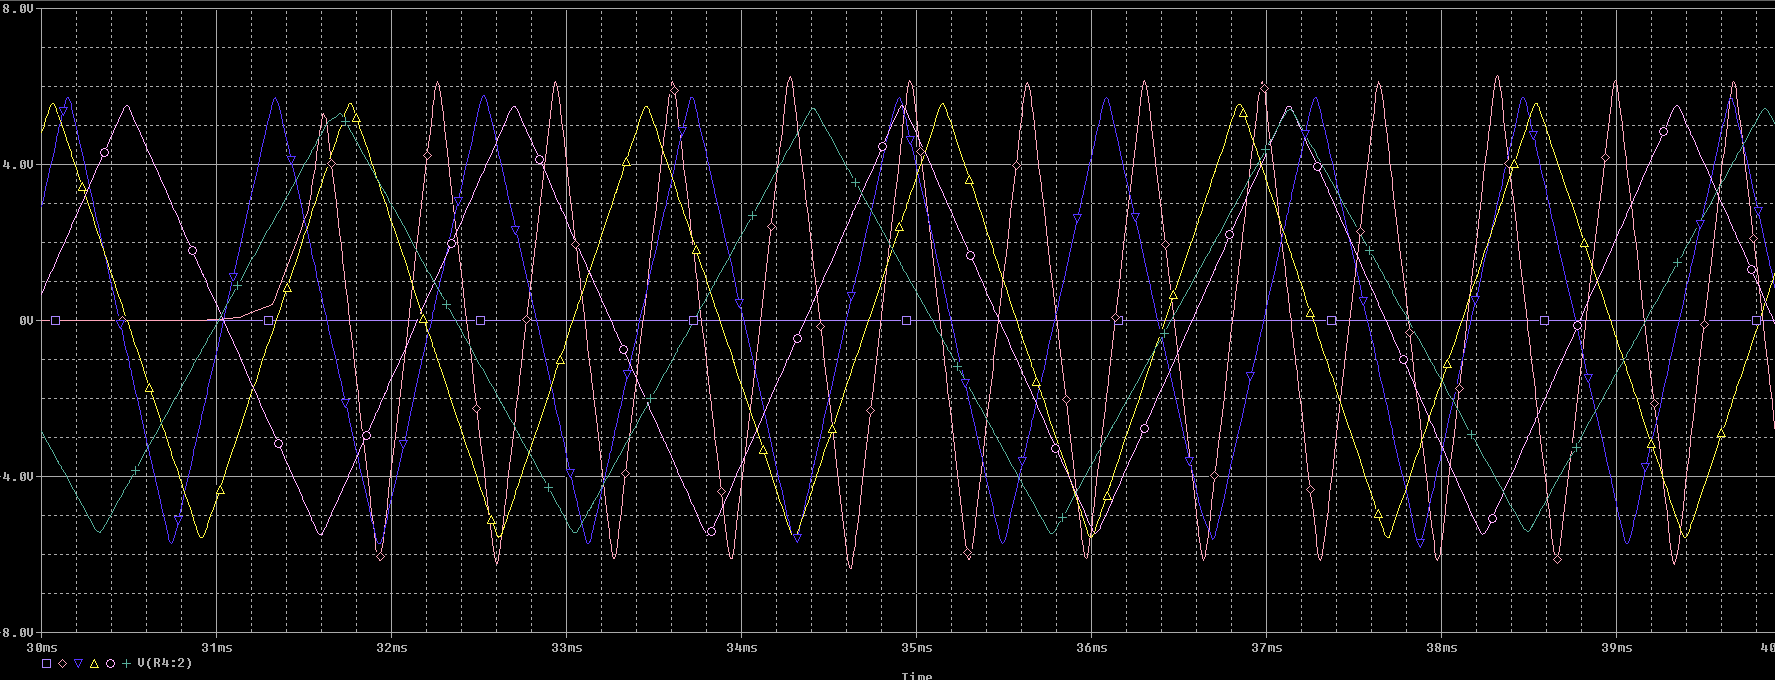
\includegraphics[width = \textwidth, height = .25\textheight, keepaspectratio]{lab/assets/gentri5.png}
    \caption{R2 = 1k}
\end{figure}

\begin{figure}[h!]
    \centering
	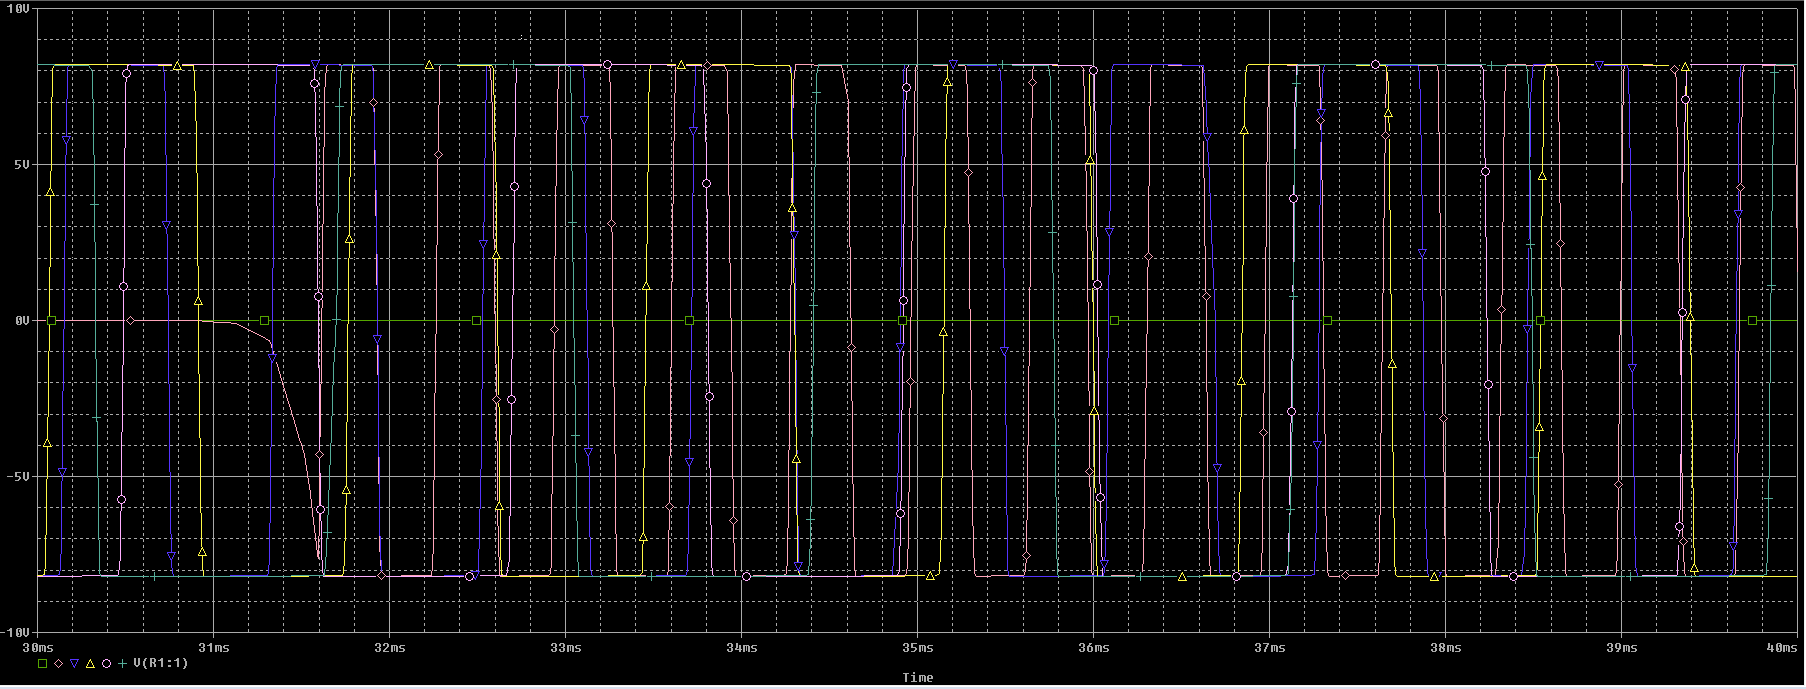
\includegraphics[width = \textwidth, height = .25\textheight, keepaspectratio]{lab/assets/gentri6.png}
    \caption{R2 = 1k}
\end{figure}

Παρατηρούμε ότι για τιμή μικρότερη της R2, ο παλμός της $V_2$ προσεγγίζει καλύτερα έναν τετραγωνικό. Αυτό συμβαίνει διότι η R2 είναι υπεύθυνη για την πτώση τάσης στην V2 της οποία η δίοδος zener πολώνεται πλέον αποτελεσματικά. Επίσης απόρροια αυτού είναι να έχουμε έναν πιο "καθαρό" τριγωνικό παλμό, οι κορυφές είναι πιο απότομες.

Με ανάλογο τρόπο με το ερώτημα 4, βλέποντας τις παραμετρικές αναλύσεις θεωρούμε ως τιμή αντίστασης που ξεκινάει η αλλοίωση την τιμή 21k. Οπότε θα έχουμε $f_{max} = 1/T_{max} = 1/0.6ms \approx 1.7kHz$. Πράγματι η μέγιστη συχνότητα εύρυθμης λειτουργίας αυξήθηκε.

\subsection{Ερώτημα 7}

Επειδή η τάση εξόδου αλλά και η περίοδος εξαρτώνται απο τον λόγο αντιστάσεων Rf και R1, για να μεταβάλουμε αποκλειστικά το πλάτος της τριγωνικής κυματομορφής θα μπορούσαμε να μεταβάλλουμε την V2 επηρεάζοντας την τάση φραγής της zener (η τρέχουσα τιμή είναι 7.5).


\section{Άσκηση 2}

Η άσκηση 2 αναφέρεται στην δημιουργία γεννήτριας κλιμακωτής τάσης. Ο ασύμμετρος ασταθής πολυδονητής Β ελέγχει την λειτουργία του ασύμμετρου ασταθή πολυδονητή  Α και του ολοκληρωτή. Ο ασταθής Α (555 timer) παράγει έναν τετραγωνικό παλμό ο οποίος είναι η είσοδος του ολοκληρωτή. Στη συνέχεια, αυτός ο παλμός φορτίζει τον πυκνωτή που είναι συνδεδεμένος στην έξοδο του ολοκληρωτή, με αποτέλεσμα να δημιουργούνται σκαλοπάτια κάθε φορά που συναντάμε στην είσοδο έναν παλμό. Αυτά τα σκαλοπάτια θα μπορούσαν θεωρητικά να συνεχίζουν την ανοδική τους πορεία μέχρι να φτάσουμε την τιμή της τροφοδοσίας. Για να μην συμβεί κάτι τέτοιο, υπεύθυνος είναι ο ασταθής Β. Ο ασταθής Β ελέγχει τα δύο τρανζίστορ (2Ν222) και απο τη μία εκφορτίζει τον πυκνωτή κατάλληλα επαναφέροντας τα σκαλοπάτια στην αρχική τους κατάσταση και απο την άλλη προκειμένου να γίνει αυτό αποτελεσματικά, κρατάει τον 555 εκτός λειτουργίας. Αξίζει να σημειωθεί ότι προκειμένου να μην έχουμε τάση στην βάση χαμηλότερη απο τον εκπομπό, χρησιμοποιούμε μια δίοδο ως ανορθωτή.

Για να ισχύουν οι προυποθέσεις της εκφώνησης έχουμε: R1 = 2886 Ω (2.7k), R2 = 54834 Ω (56k), Ra = 18181 Ω (18k), Rb = 163636 Ω (150k).

\begin{figure}[h!]
    \centering
	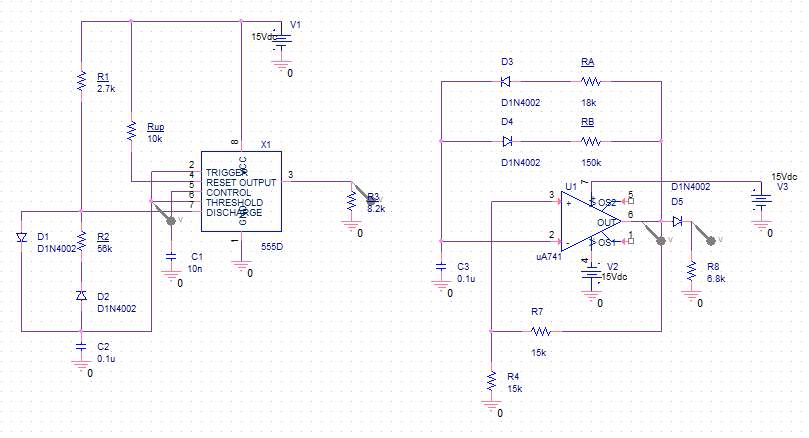
\includegraphics[width = \textwidth, height = .25\textheight, keepaspectratio]{lab/assets/circuit_pre.png}
	\caption{Κυκλώματα των ασταθών Α και Β}
\end{figure}

\subsection{Ερώτημα 3}
\begin{figure}[h!]
    \centering
	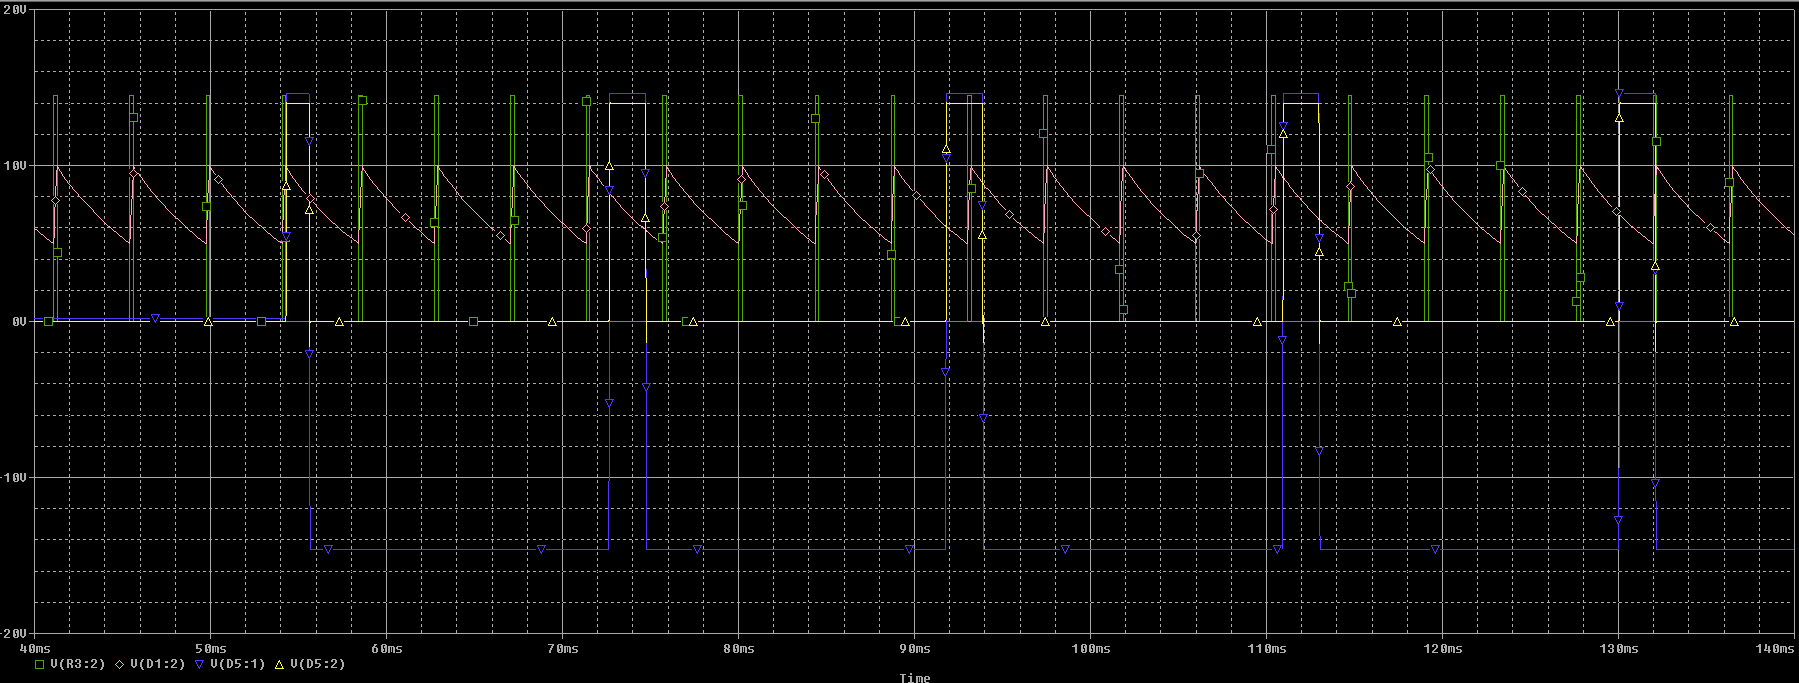
\includegraphics[width = \textwidth, height = .25\textheight, keepaspectratio]{lab/assets/voltage_step1.png}
	\caption{Οι κυματομορφές των V1, ακροδέκτης 6 του 555 και V2 και V3}
\end{figure}

Παρατηρούμε ότι η δίοδος κάνει σωστά την δουλειά της και κόβει τις αρνητικές τιμές τάσεις.

\subsection{Ερώτημα 4}


\begin{figure}[h!]
    \centering
	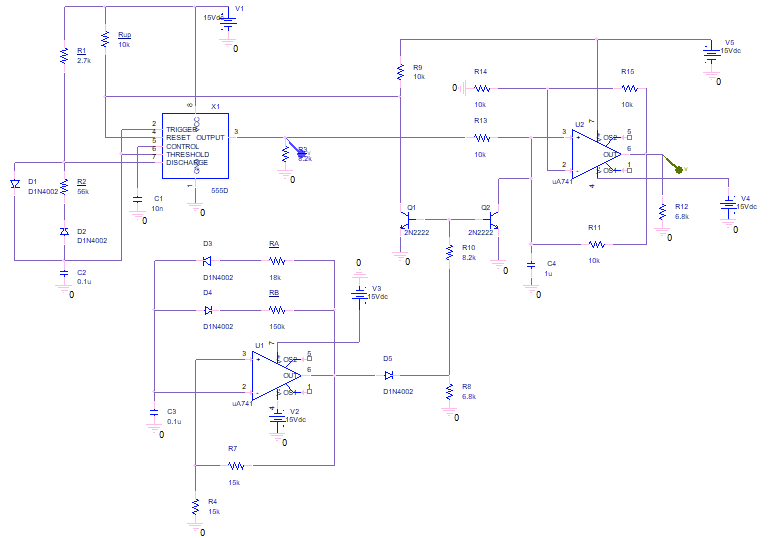
\includegraphics[width = \textwidth, height = .4\textheight, keepaspectratio]{lab/assets/circuit_full.png}
	\caption{Ολικό κύκλωμα. Πλέον συνδέσαμε και τον ολοκληρωτή}
\end{figure}


\begin{figure}[h!]
    \centering
	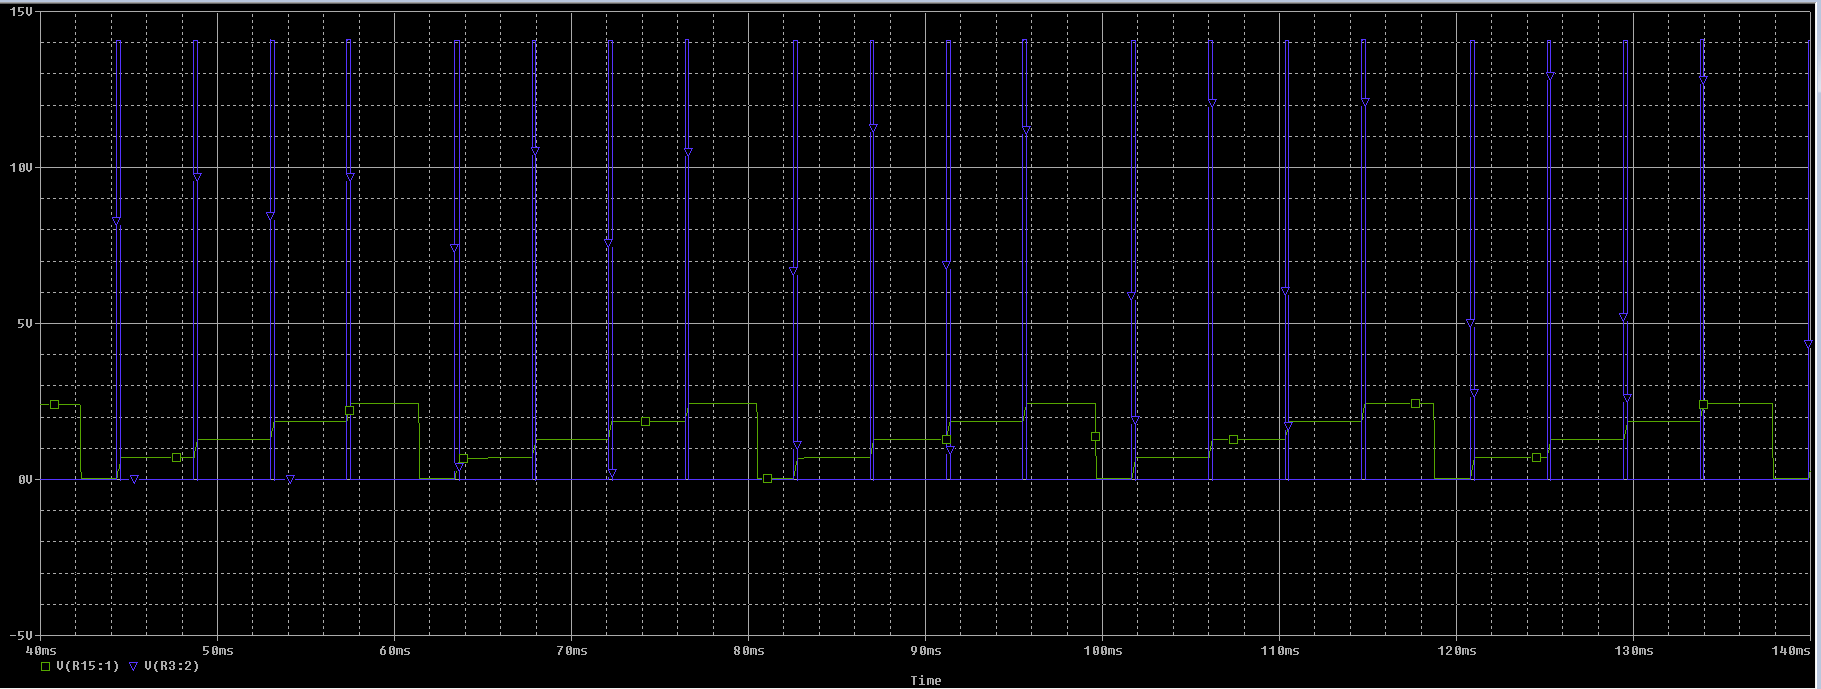
\includegraphics[width = \textwidth, height = .4\textheight, keepaspectratio]{lab/assets/v1_vout.png}
	\caption{Οι κυματομορφές των V1 και Vout}
\end{figure}

Επιτυχώς βλέπουμε την κλιμακωτή τάση και τα σκαλοπάτια αλλά και την επαναφορά τους.

\end{document}